\documentclass[]{article}
\usepackage[english,ngerman]{babel}
\usepackage[utf8]{inputenc}
\usepackage{listings}
\usepackage{graphicx}
\linespread{1.2}

\usepackage{listings}
\usepackage{xcolor}
\usepackage{color}
\usepackage{amsmath}
\usepackage{amssymb}
\usepackage[babel,german=quotes]{csquotes}

\definecolor{dkgreen}{rgb}{0.1,0.4,0.1}
\definecolor{gray}{rgb}{0.5,0.5,0.5}
\definecolor{mauve}{rgb}{0.58,0,0.82}
\definecolor{listinggray}{gray}{0.9}
\definecolor{lbcolor}{rgb}{0.9,0.9,0.9}
\definecolor{mygray}{rgb}{0.4,0.4,0.4}
\definecolor{mygreen}{rgb}{0,0.8,0.6}
\definecolor{myorange}{rgb}{1.0,0.4,0}

\lstset{
	%backgroundcolor=\color{lbcolor},
	tabsize=4,    
	%   rulecolor=,
	language=C,
	basicstyle=\scriptsize,
	%upquote=true,
	aboveskip={1.5\baselineskip},
	columns=fixed,
	%showstringspaces=false,
	extendedchars=false 
	breaklines=true,
	prebreak = \raisebox{0ex}[0ex][0ex]{\ensuremath{\hookleftarrow}},
	%frame=single,
	numbers=left,
	showtabs=false,
	showspaces=false,
	showstringspaces=false,
	emphstyle=\color{myorange},
	keywordstyle=\color[rgb]{0,0,1},
	commentstyle=\color{dkgreen},
	stringstyle=\color[rgb]{0.327,0.126,0.341},
	stringstyle=\tiny,
	numberstyle=\color[rgb]{0.205, 0.142, 0.73},
}

%opening
\title{Bierfass-Simulation}
\author{Mark Geiger \and Rico Fritzsche}

\begin{document}

\maketitle

\begin{abstract}
Im Kurs Parallele Programmierung soll eine Simulation implementiert werden, welche das Abkühlen eines Fasses darstellt. Das Fass soll in einem Eimer mit Null Grad Celsius kaltem Wasser so tief eingetaucht werden, das die Durchschnittstemperatur nach genügend langer Zeit Zehn Grad Celsius beträgt. Eine Grafik soll das Ergebnis darstellen. 
\end{abstract}

\section*{Umsetzung}
Für die Simulation wird eine Matrix definiert, welche in drei Bereiche geteilt wird. Einen Rand, welcher an jeder Seite aus einer Reihe besteht. Hier werden die Außentemperaturen festgelegt. Der äußere Bereich wird dazu nochmals horizontal geteilt, was die Eintauchtiefe des Fasses umsetzt. Dem oberen Teil des Randes wird die Außentemperatur zugewiesen, in unserem Fall 30 Grad Celsius. Der untere Teil erhält den Wert Null Grad Celsius, welches die Temperatur des Wasser in dem Eimer entspricht. Das innere wird mit einer beliebigen Ausgangstemperatur belegt. \\
Damit die Threads bei der Berechnung sich nicht gegenseitig Behindern und falsche Werte berechnen, wird eine Schreib- und eine Lesematrix initialisiert. Anschließend wird die gewünschte Anzahl an Threads gestartet, in unserem Beispiel 200. Diese führen die Berechnung nach folgendem Muster aus. Jeder Thread wählt einen zufälligen Punkt in der Matrix den er im Zyklus bearbeitet. Ist der gewählte Punkt eine Randpunkt, startet er einen neuen Zyklus. Trifft er einen Punkt innerhalb des Randes (im Fass), holt er sich die Werte der umliegenden Punkte aus der Lesematrix. Aus diesen bildet er den Durchschnitt und schreibt das Ergebnis an die Stelle des zu Beginn gewählten Punktes in die Schreibmatrix. Anschließend beginnt ein neuer Zyklus. Der beschriebene Algorithmus wird in Listing 1 abgebildet.

\begin{lstlisting}
void step(){   
	int size = SIZE;
	
	while(finished == FALSE){
		int c,d;
		c = rand() % (size-2)+1;
		d = rand() % (size-2)+1;
		
		if (isPointWarm(c,d)) {
			writeMat[c + d * SIZE] =  WARM_TEMP;
		} else if(isPointCold(c,d)) {
			writeMat[c + d * SIZE] = COLD_TEMP;
		} else {
			double z1 = readMat[c + 1 + d * size];
			double z2 = readMat[c - 1 + d * size];
			double z3 = readMat[c + (d - 1) * size];
			double z4 = readMat[c + (d + 1) * size];
			double z5 = readMat[c + d * size];
			double z6 = readMat[c + 1 + (d - 1) * size];
			double z7 = readMat[c - 1 + (d + 1) * size];
			double z8 = readMat[c - 1 + (d - 1) * size];
			double z9 = readMat[c + 1 + (d + 1) * size];
			writeMat[c + d * SIZE] = (z1 + z2 + z3 + z4 + z5 +
			 z6 + z7 + z8 + z9) / 9.0;
		}
	}
}
\end{lstlisting}

Im Mainthread werden nach kurzer Wartezeit die Ergebnisse der Schreibmatrix in die Lesematrix kopiert. Damit rechnen die Threads mit etwas Verzug mit den aktuellen Temperaturwerten. \\
Zur Visualisierung wird die Schreibmatrix beim kopieren in die Lesematrix zusätzlich in eine Textdatei kopiert. Nach Beendigung des Programms liest ein Python-Skript die Dateien ein und erstellt eine Colour-Map für jede gespeicherte Matrix. Abschließend können die erstellten Colour-Maps zu einer Gif-Datei zusammengefügt. In der Abbildung \ref{pic:ergebnis} ist das Endergbnis in einer Clour-Map aufgetragen. 


\section*{Ausführung}
\textit{make} (baut erste Implementation -> die bessere) \\
\textit{make main2} (um 2. Implementation zu bauen) \\
\textit{make plot} (nur möglich wenn in main2 matrizen geschrieben werden, siehe const WRITE\_RESULTS)

\newpage
\section*{Visualisierung}
\begin{figure}[h]
	\centering 
	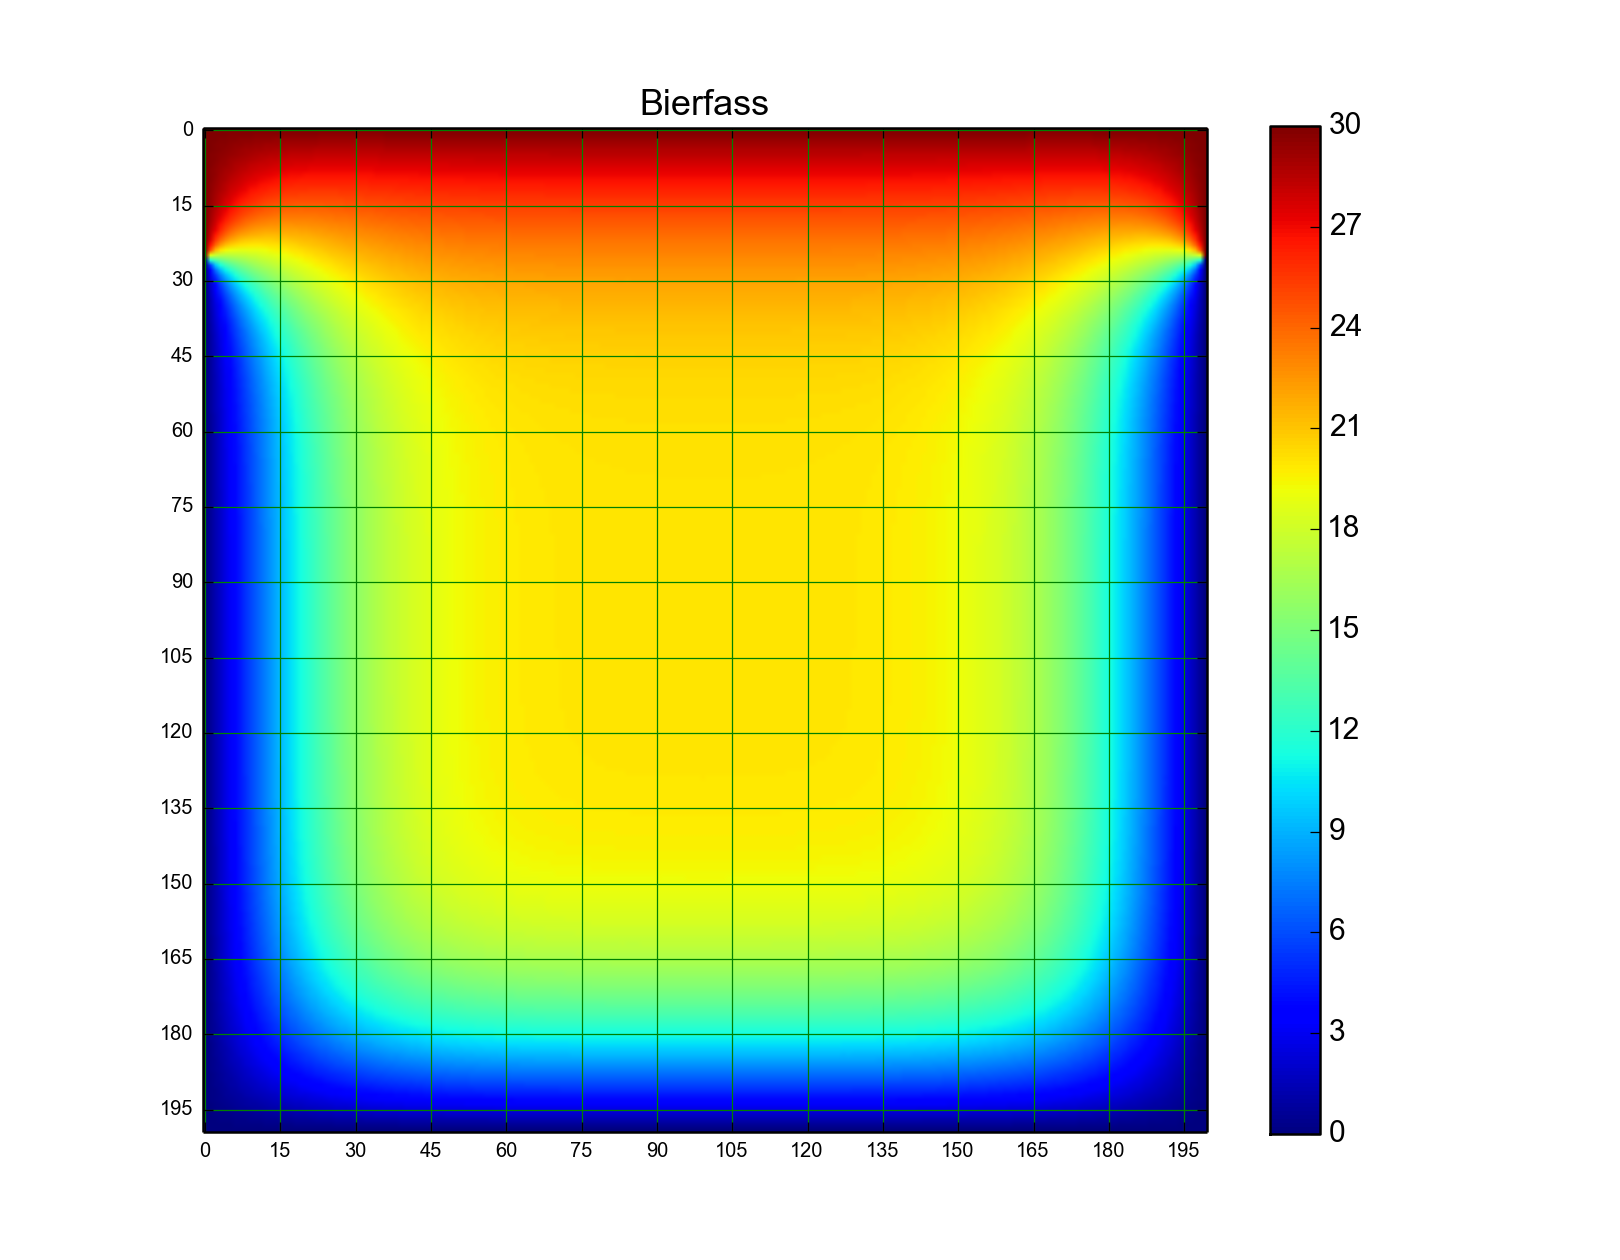
\includegraphics[width=1\linewidth]{ergebnis.png}
	\caption{Ergebnis der Testimplementation, dargestellt mittels Python-Scripts}
	\label{pic:ergebnis}
\end{figure}
\end{document}
